
%%%%%%%%%%%%%%%%%%%%%%% file typeinst.tex %%%%%%%%%%%%%%%%%%%%%%%%%
%
% This is the LaTeX source for the instructions to authors using
% the LaTeX document class 'llncs.cls' for contributions to
% the Lecture Notes in Computer Sciences series.
% http://www.springer.com/lncs       Springer Heidelberg 2006/05/04
%
% It may be used as a template for your own input - copy it
% to a new file with a new name and use it as the basis
% for your article.
%
% NB: the document class 'llncs' has its own and detailed documentation, see
% ftp://ftp.springer.de/data/pubftp/pub/tex/latex/llncs/latex2e/llncsdoc.pdf
%
%%%%%%%%%%%%%%%%%%%%%%%%%%%%%%%%%%%%%%%%%%%%%%%%%%%%%%%%%%%%%%%%%%%


\documentclass[runningheads,a4paper]{llncs}

\usepackage{amssymb}
\setcounter{tocdepth}{3}
\usepackage{graphicx}

\usepackage{url}   
\newcommand{\keywords}[1]{\par\addvspace\baselineskip
\noindent\keywordname\enspace\ignorespaces#1}

\usepackage[utf8x]{inputenc}
\usepackage[L7x]{fontenc}
\usepackage[lithuanian]{babel}

\begin{document}

\mainmatter  % start of an individual contribution

% first the title is needed
\title{Optimalių maršrutų paieškos algoritmai}

% a short form should be given in case it is too long for the running head
\titlerunning{Optimalių maršrutų paieškos algoritmai}

% the name(s) of the author(s) follow(s) next
%
% NB: Chinese authors should write their first names(s) in front of
% their surnames. This ensures that the names appear correctly in
% the running heads and the author index.
%
\author{Karolis Šarapnickis}
%
\authorrunning{Optimalių maršrutų paieškos algoritmai}
% (feature abused for this document to repeat the title also on left hand pages)

% the affiliations are given next; don't give your e-mail address
% unless you accept that it will be published
\institute{Kompiuterijos katedra, Vilniaus universitetas, Lietuva}

%
% NB: a more complex sample for affiliations and the mapping to the
% corresponding authors can be found in the file "llncs.dem"
% (search for the string "\mainmatter" where a contribution starts).
% "llncs.dem" accompanies the document class "llncs.cls".
%

\toctitle{Optimalių maršrutų paieškos algoritmai}
\maketitle


\begin{abstract}
Darbe analizuojamos genetinio algoritmo modifikacijos sprendžiant modifikuotą keliaujančio pirklio uždavinį.
\keywords{Keliaujančio pirklio problema, Hamiltono ciklas, genetinis algoritmas, skruzdėlių kolonijos algoritmas, simuliuoto atkaitinimo algoritmas}
\end{abstract}


\section{Įvadas}

Optimalių maršrutų paieškos aktualumas kiekvieno iš mūsų kasdieniniame gyvenime buvo aptartas pirmame moksliniame tiriamajame darbe. Jame buvo susipažinta su keletų heuristinių optimalaus maršruto paieškos algoritmų ir spręstos keliaujančio pirklio problemos pilno grafo atveju \cite{mtd1}.

Yra nemažai mokslinių darbų sprendžiančių keliaujančio pirklio problemas naudojant heuristinius algoritmus, juos modifikuojant ir parenkant įvairiausias sąlygas. Tačiau didžioji dali tokių darbų analizuoja pilnus grafus (kiekvienas miestas turi tiesioginį kelią su bet kuriuo kitu miestu), o realiame gyvenime praktiškai nėra didesnių sausumos žemėlapių, kuriuose kiekvienas miestas būtų tiesiogiai susietais keliais su likusiais miestais.

Šio mokslinio darbo tikslas yra naudojant heuristinius algoritmus ir jų modifikacijas ieškoti trumpiausio maršruto tarp miestų aplankant juos bent vieną kartą. Visi analizei naudojami grafai yra panašūs į sausumos miestų žemėlapius – juose įmanoma aplankyti visus miestus, o grafo kraštinės niekur nesusikerta.


\subsection{Panašūs darbai}

Genetiniai algoritmai pradėti naudoti sprendžiant keliaujančio pirklio uždavinį jau nuo 1990m. Genetinio algoritmo modifikacijos ir jo hibridai taip pat pradėti taikyti jau nuo 2005m. Didžioji dalis straipsnių sprendžiančių optimalaus maršruto problemą ieško pilno Hamiltono ciklo. Šiame moksliniame darbe miestą galima aplankyti daugiau negu vieną kartą. Todėl iš esmės taikomi metodai nėra nauji, tačiau jų pritaikymas pasirinktai problemai nėra niekur publikuotas.

\section{Dėstymas}


\subsubsection{Genetinis algoritmas.}

Genetiniai algoritmai (GA) (angl. genetic algorithm) – vieni iš heuristinių algoritmų, įkvėptų gamtos. Jie yra paremti evoliuciniu gamtos modeliu, kai keičiantis kartoms individai tampa vis tobulesni ir labiau prisitaikę prie aplinkos sąlygų.

Dėl keliaujančio pirklio problemos paprastos formuluotės yra bandoma įvairiausius algoritmus panaudoti sprendžiant šią problemą. Ne išimtis yra ir šie algoritmai, tačiau „grynieji“ genetiniai algoritmai, kurti J. H. Holland'o ir jo studentų Mičigano universitete 60-taisiais, 70-taisiais, nebuvo sugalvoti spręsti kombinatorinio optimizavimo problemas. Tai laikais genetiniai algoritmai dažniausiai buvo naudojami spręndžiant įvairias skaitines funkcija, todėl norint rasti keliaujančio pirklio problemos sprendimą, reikia atlikti tam tikrus genetinio algoritmo pakeitimus \cite{genetictsp}.

Genetinis algoritmas iš esmės operuoja su baigtine chromosomų arba bitų sekų populiacija. Paieškos mechanizmas susideda iš trijų skirtingų fazių: kiekvienos chromosomos tinkamumo (angl. fitness) įvertinimas, tėvinių chromosomų parinkimas ir mutacijos bei rekombinacijos operatorių pritaikymas tėvinėms chromosomoms. Naujos chromosomos, gautos pritaikius genetinius operatorius, dalyvauja tolimesnėje revoliucijos iteracijoje ir pati sistema tobulėja augant kartų skaičiui \cite{genetictsp}.

\medskip

\noindent
{\it Genetinės sistemos supaprastintas pseudo-kodas}
\begin{verbatim}
    1. Sukuriama pradinė P chromosomų populiacija (0 karta).
    2. Įvertinamas kiekvienos chromosomos tinkamumas.
    3. Pasirenkama P tėvų iš esamos populiacijos pasitelkiant proporcingumo 
        taisykle (angl. proportional selection) (pasirinkimo tikimybė priklauso nuo 
        tinkamumo vertės).
    4. Dauginimuisi atsitiktinai pasirenkama pora chromosomų. Atliekama 
        rekombinacijos operacija apkeičiant bitus pasirinktame taške, taip sukuriant 
        vaikines chromosomas.
    5. Kiekviena vaikinė chromosoma apdorojama mutacijos operatoriais ir 
        grąžinama į populiaciją.
    6. Kartojami 4 ir 5 žingsniai kol visos chromosomos būna parinktos ir 
        paveiktos genetiniais operatoriais.
    7. Sena chromosomų populiacija pakeičiama nauja.
    8. Įvertinamas kiekvienos chromosomos tinkamumas.
    9. Kartojama viskas nuo 3 žingsnio kol pasiekiamas atitinkamas kartų 
        skaičius ar kitokia sąlyga.
\end{verbatim}
%
\noindent
{\small Genetinio algoritmo pseudo-kodas \cite{genetictsp}.}


\subsection{Eksperimentinė dalis}

Hibridiniu genetiniu algoritmu buvo sprendžiama modifikuota keliaujančio pirklio problema grafuose, kurie neturi pilno Hamiltono ciklo. Dėl pastarosios sąlygos keliaujančio pirklio problemos taisyklė, kad kiekvienas miestas turi būti aplankytas tik vieną kartą, buvo pakeista leidžiant kiekvieną miestą aplankyti daugiau negu vieną kartą. Tokios analizės krypties išvados yra plačiau pritaikomos sprendžiant praktinius optimaliausių maršrutų uždavinius.

Daugelis heuristinių algoritmų turėdami neribotą laiką galėtų rasti optimaliausią maršrutą. Tačiau skaičiavimo laikas yra ne ką mažiau svarbesnis matavimo vienetas už patį maršruto ilgį. Taip pat tokie algoritmai pasižymi įsisotinimu ties tam tikromis ribomis, ties kuriomis maršruto trumpėjimas labai sustoja. Todėl mokslinio darbo metu buvo ieškoma ne tik optimalių parametrų su kuriais būtų gaunamas geriausias vidutinis rezultatas, bet ir su kokiais parametrais kokiose algoritmo gyvavimo laikotarpiuose maršrutas trumpėja greičiausiai.

Programinis kodas parašytas naudojant Python 2.7 programinę kalbą ir vykdytas Ubuntu operacinėje sistemoje.

\begin{figure}
\centering
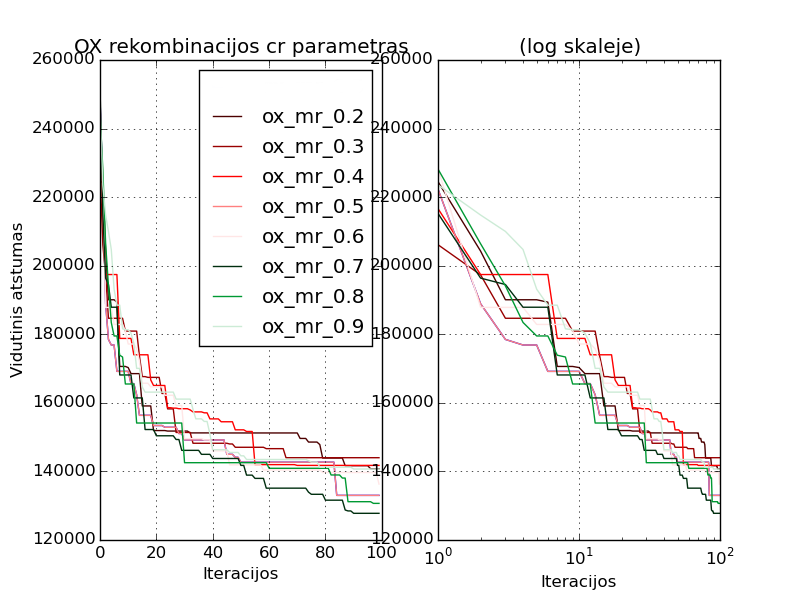
\includegraphics[height=8.2cm]{img/cros}
\caption{Rekombinacijos koeficiento įtaka trumpiausio maršruto paieškai.}
\label{fig:cros}
\end{figure}

~\ref{fig:cros} pav. matyti kad naudojant 0.7-0.8 rekombinacijos koeficientą su OX rekombinacija pasiekiami geriausi rezultatai analizuojant 80 miestų grafą. Tačiau analizuojant 44 miestų grafą geresni rezultatai pasiekti su 0.3-0.4 koeficientais.

\begin{figure}
\centering
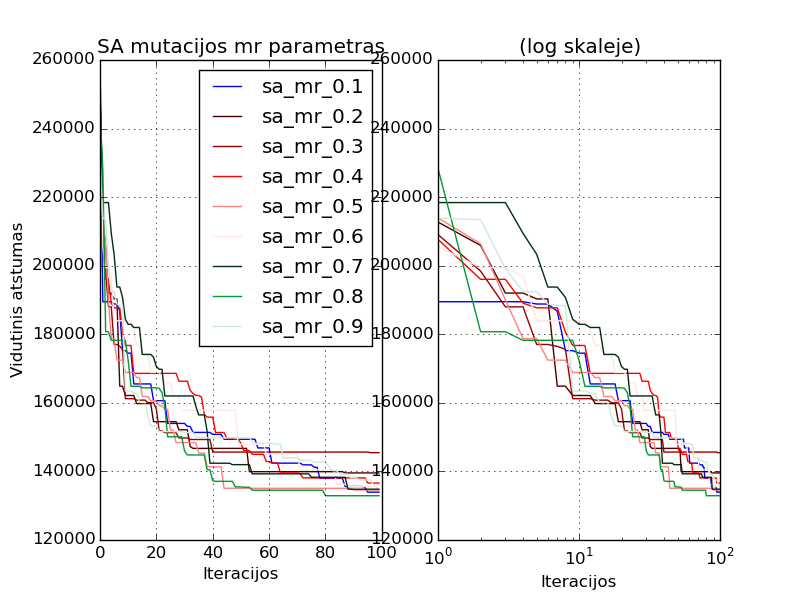
\includegraphics[height=8.2cm]{img/mut}
\caption{Mutacijos koeficiento įtaka trumpiausio maršruto paieškai.}
\label{fig:mut}
\end{figure}

Analizuojant mutacijos koeficientą (~\ref{fig:mut} pav.) taip pat pastebėta, kad su skirtingais grafais optimalus mutacijos koeficientas skiriasi, tačiau tas skirtumas yra kur kas mažesnis. Todėl pastebėta, kad optimalus mutacijos koeficientas yra nuo 0.5 iki 0.8.

\begin{figure}
\centering
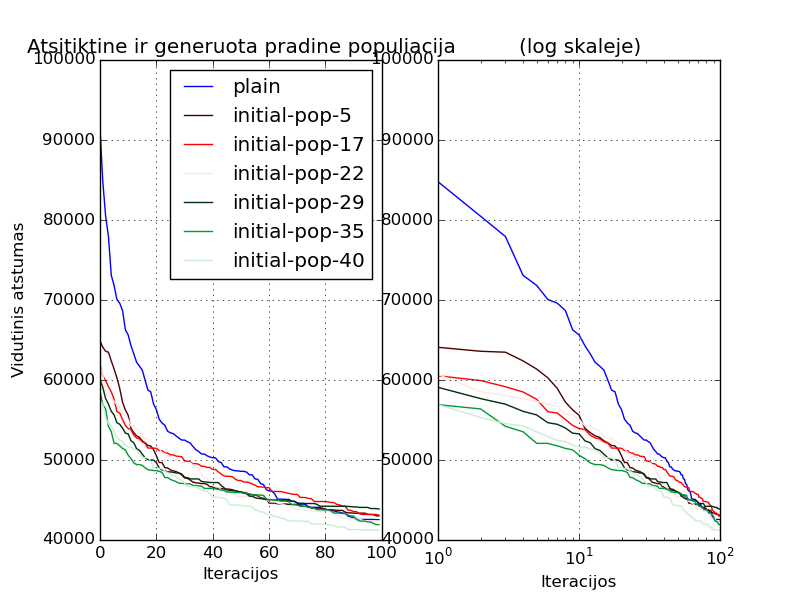
\includegraphics[height=8.2cm]{img/pop}
\caption{Atsitiktinių ir su skruzdėlių kolonijos algoritmų generuotų pradinių populiacijų įtaka trumpiausio maršruto paieškai.}
\label{fig:pop}
\end{figure}

Analizuojant pradinės populiacijos įtaka (~\ref{fig:pop} pav.) visais grafų atvejais pastebimas reultatų pagerėjimas kaip apie 60\% pradinės populiacijos generuojama hibridiniu skruzdėlių kolonijos algoritmu.

\subsubsection{Praktinis uždavinys.}

Kadangi iki šiol analizuoti grafai buvo praktiškai sintetiniai (atsitiktinai sugeneruoti ir modifikuoti ranka) ir gauti parametrų rezultatai yra pastebimai įtakojami grafų pavidalo, buvo nuspręsti išanalizuoti parametrų įtaką nagrinėjant praktinį uždavinį.

Sukurtas genetinio algoritmo hibridas ir jo implementacija buvo pritaikyta ieškant trumpiausio maršruto siekiant apvaikščioti visas Vilniaus senamiesčio gatveles (~\ref{fig:vln} pav.).

\begin{figure}
\centering
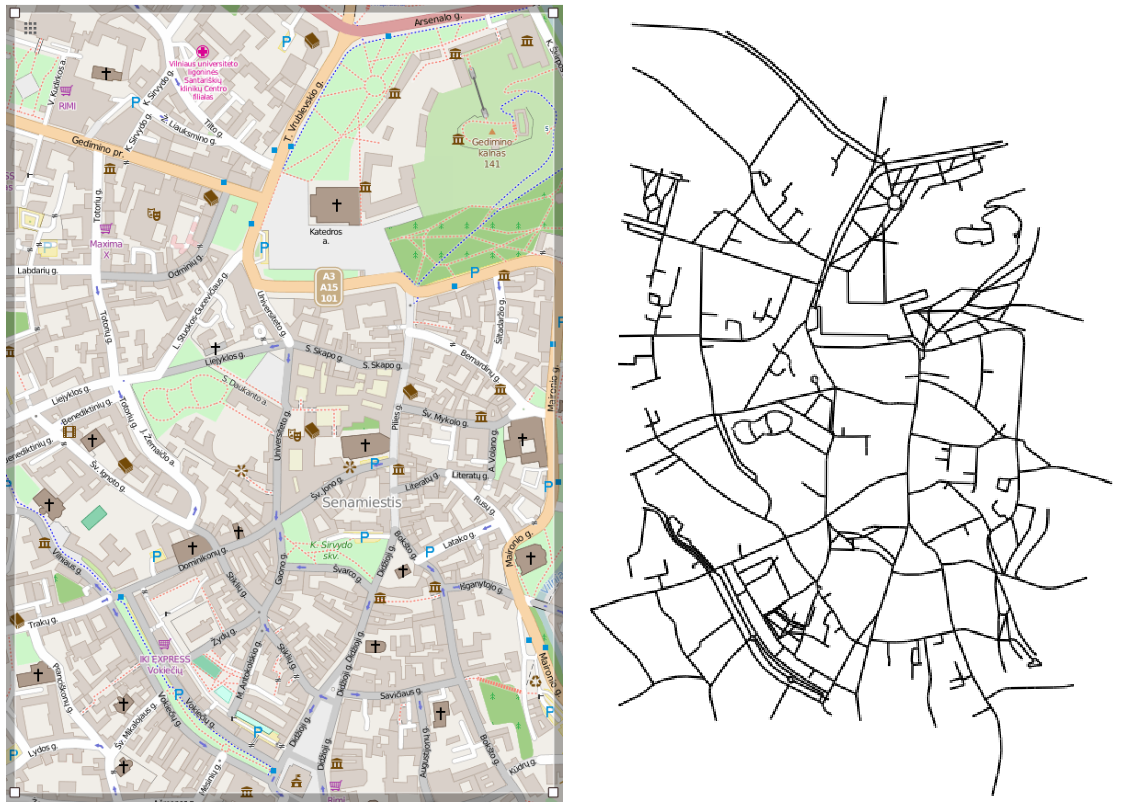
\includegraphics[height=8.2cm]{img/vln}
\caption{Vilniaus senamiesčio žemėlapis (kairėje) ir jo pavidalas grafe (dešinėje).}
\label{fig:vln}
\end{figure}


\section{Išvados}

Dalį pradinės genetinio algoritmo populiacijos pakeitus hibridiniu skruzdėlių kolonijos algoritmu generuotomis chromosomomis yra gerokai pagerinami algoritmo rezultatai.

Grafų struktūra geroaki įtakoja mutacijos ir rekombinacijos efektyiausius koeficientus, nors iš turimų rezultatų būtų galima teigti, kad optimaliausias mutacijos koeficients yra nuo 0.5 iki 0.8.



\begin{thebibliography}{4}

\bibitem{mtd1} Šarapnickis, K.: Mokslo tiriamasis darbas II: optimalių maršrutų paieškos algoritmai, (2015)

\bibitem{genetictsp} Potvin, J. Y.: Genetic algorithms for thetraveling salesman problem, (1996)

\bibitem{genetic_hybrid} Shyi-Ming C., Chih-Yao C.: Solving the traveling salesman problem based on the genetic simulatedannealing ant colony system with particle swarm optimization techniques, (2011)

\end{thebibliography}


\end{document}
